\chapter{Model validation}
\label{ch:valid}


The previous sections have introduced a plethora of data models which could be used as tools for answering questions using data. However, we have only briefly touched upon a discussion of the different methods of model validation, or assessing how well these models are fitting the data, a step that is too often ignored. Further, the process of model validation tends to go hand-in-hand with the notion of model selection: identifying which model is the ``best'' among a set of possible candidates. Without model validation, there is no reason to trust the conclusions drawn. In this section we will begin with discussion various approaches to model validation and finally will move onto the relationship to model selection.



\section{Visualization}

Visualization of data is an extremely useful way to validate that a procedure is working well. If we can examine the data with our own eyes, we are much more likely to obtain an accurate understanding of the structure of the data and be able to evaluate the results of our models.

\subsection*{Residual plots}

If we can visualize the data, for example by plotting residuals against a variable of interest or the fitted values, then we can get a feel for where a linear model works well and where it does not. Recall our discussion of residual plots in our section on linear models. The patterns of the residuals give helpful clues about whether the model is fitting the data well. For example, residuals randomly scattered about zero indicate that the model fits well, whereas residuals whose variance increases as the fitted values (or a variable of interest) get larger/smaller, is indicative of \textit{heteroskedasticity}, or non-constant variance, in the data (perhaps we should have fit the linear model using generalized least squares instead!)



\section{Prediction}


If a linear or classification model produces accurate predictions, then it is likely that the model is capturing some of the underlying mechanisms that exist in the data generation process. Although there exist a number of methods often considered to be ``uninterpretable'' or are known to be biased that provide better predictions than the more interpretable models. For classification models, we typically assess the quality of predictions using the classification error on an independent test set (a subset of the data that was not used to define the model); the proportion of observations that are misclassified.

$$\text{classification error } = \frac{\#\{\text{false positives}\} + \#\{\text{false negative}\}}{\#\{\text{test samples}\}}$$

where a false positive is the case where the predicted class/response is $\hat{y} = 1$ but the true class is $y = 0$, and a false negative is the case where the predicted class is $\hat{y} = 0$ but the true value is $y = 1$.

For a model with a continuous response (such as a linear model), we typically look at the residual sum of squares (RSS); a measure of the difference between the predicted values and the true values. For example, suppose we have a linear model $y =  X\beta + \epsilon$, then the predicted values are given by $\hat{y} = X \hat{\beta}$, and the RSS is given by

$$RSS = \sum_{i=1}^n (\hat{y}_i - y_i)^2$$

however, again, ideally we would calculate the corresponding sum of squares using an independent test set, rather than the original observations.



\section{Interpretability}

If our model can be shown to have a meaningful interpretation, then we might be more inclined to accept its results. For example, suppose that we were conducting an experiment to identify genes that differ between cancer patients and healthy patients and we found that a particular subset of genes had a significantly different expression pattern in the cancer patients than the healthy patients. If domain experts were already aware that at least some of these genes were biologically meaningful (for example they were already known to play a role in the progression or development of the particular cancer), then it would not be unreasonable to postulate that the other genes found to differ significantly between the two groups are also important. That is, we have used the domain knowledge confirmation that some of our results are meaningful to provide credence to the notion that the other results might be too. Applied statisticians are encouraged to communicate with domain experts to identify whether their results are meaningful. An idea is to show the domain experts, not just your results, but also manipulated results (for example by selecting random gene names) and let them choose which list is more meaningful. This kind of approach can be used to ensure that your domain knowledge collaborators are not simply finding interpretations of your results because they tend to see what they want to see, or want to find results where there are none.

\section{Replication of results}

Perhaps one of the most important techniques for validation of results is to replicate the results in an independent setting. Unfortunately, there are many naive approaches to ``replication'' which can provide a misleading sense of confidence; primarily when the validation is performed using the same data that was used to generate the model or draw the conclusions. This is an example of \textit{data snooping}, another example of which is to use a dataset to fish for interesting facts and then subsequently use the same dataset to prove these facts! Data snooping often leads to overfitting of models, high false positive rates and selective simulation results (choosing the simulation results that look the best, but are not necessarily representative).

How can we avoid data snooping? Probably the best is to have another lab or group replicate the experiment by generating completely new data and performing their own analysis. If they independently arrive at the same conclusions, then we have stronger evidence in favor of the validity our conclusions and models. Unfortunately, however, in most situations it is impractical to have others independently repeat our experiments. For this reason, it is good practice to use a test set of data points (or set aside a test set from our overall dataset) so that we can use this test data at a later date to validate the conclusions drawn and models developed from the remaining training data. In general, it is recommended that exploratory data analysis and confirmatory data analysis should be done on separate datasets if possible, otherwise the best approach is to perform these tasks on separate subsets of the original dataset.



\section{Robustness}

Ideally our conclusions and methods should be robust both to the specific samples used as well as departures from model assumptions.

\subsection*{Robustness to sampling}

One approach to identifying whether or not your results are nonsense is to perturb the data (for example by re-sampling and using various different random subsets of the data) and re-evaluate your results or re-fit your model. If you are obtaining equivalent results on the perturbed data, then this means that the results were not dependent on the specific set of observations used (this is a good thing!). If however your results are extremely variable based on which subset of the data you use, then this should lead you to be heavily suspicious of the results. If this is the case, then it is likely that the particular model being used is not yielding robust or reliable results, and you should search for alternative methods.

\subsection*{Robustness to assumptions}

There is also the question of how robust our conclusions are to the assumptions of the model used. For example, if the model assumes normality, how reasonable are our conclusions when our data is not \textit{exactly} normal? For most commonly used methods, there exist a lot of work describing the effect of departures from the base assumptions. For example, it is known that $t$-tests are somewhat robust to the normality assumption (particularly for large sample sizes), whereas $F$-tests are not. It is thus important to assess not only whether your data satisfies the required assumptions of your analysis, but also, if there are indeed slight deviations, to assess whether this has significantly affected the conclusions drawn. If the effects of departures from the model assumptions are not known for the method at hand, then it might be an idea to conduct some simulations.


\section{The likelihood ratio test}

A more traditional approach to model checking is to perform a \textit{likelihood ratio test} (often referred to as an $F$-test in the regression literature). For a saturated model (a model which has as many parameters as there is information in the data), suppose that $y_i \sim Binomial(\pi_i, n_i)$. Then we estimate

$$\tilde{\pi}_i  = \frac{y_i}{n_i}$$

where  with $n_i$ not too small. 



\section{Model selection}

Above we have discussed many approaches to identifying whether a model is ``valid'', the meaning of which is left up to the user based on their overall reason for generating the model in the first place. However, we have not discussed how such tools allow us to compare different models in order to identify which is the ``best''. We note however, that in most cases, there is no single best model, rather, the model ranking will depend significantly on what is we would like it to be the best at. For example, do we want to find the model that produces the most accurate predictions, the model that is the most interperatable, the model that is the least variable, a combination of these or something else entirely?

There exist a number of formally defined metrics which can be used to compare one model to another. In fact, we have already discussed some examples above: we could define the best model to be that which obtained the minimum residual sum of squares or prediction error.

\subsection*{Kullback-Leibler Divergence}

Suppose that the true model that represents the relationship between the predictor variables, $X$, and the response variable, $y$, is defined by $y = f(X)$. Crucially, we do not know what $f$ is; we don't even know what kind of form it might take. What we can do is come up with a number of plausible models, $g_1(X|\theta_1), ..., g_K(X|\theta_K)$, each of which we could use to approximate the true model. How could we identify which of these $K$ models is the ``closest'' to $f$? First, how do we even define a notion of distance between two models? There are a number of possible distance metrics (for example, we could simply use the prediction error), however, we will focus, for the moment, on something called the Kullback-Leibler divergence (KL-divergence), which, for two functions or more specifically for two probability density functions, $f$ and $g$, is defined by

\begin{align}
\label{eq:KL}
D_{KL}(f || g) &= \int f(x) \log \frac{f(x)}{g(x)} dx \notag\\
& = \int f(x) \log f(x) dx - \int f(x) \log g(x) dx \notag \\
& = \int f(x) \log f(x) dx - E_{f} \log g(X)
\end{align}

where $E_f(h(X)) = \int h(x) f(x) dx$ denotes the expected value of $h(X)$ when $X$ has density given by $f$. It is important to note that the definition of KL-divergence is not symmetric, i.e. $D_{KL}(f || g) \neq D_{KL}(g || f)$ (so KL-divergence is not technically a metric in the traditional sense).

Thus, if we were interested in identifying which of our models, $g$, has the minimal KL-divergence from the true model $f$, we need to identify

$$\underset{m}{\text{argmin}} ~D_{KL}(f || g_m(x | \theta^*_m)~, ~~~~~~~~~~~m = 1, ..., K$$

where, since for each model, the parameters $\theta_1, ..., \theta_K$ need to be estimated, we find the optimal $\theta_1, ..., \theta_K$ by

$$ \theta^*_m = \underset{\theta}{\text{argmin}}~D_{KL}(f || g_m(x | \theta))~, ~~~~~~~~~~~m = 1, ..., K$$

In other words, expressing the KL-divergence as in \ref{eq:KL}, to identify the optimal model we need to calculate

$$\underset{m}{\text{argmax}} \left[ E_Y E_X \log (g_m(X | \hat{\theta}(y))) \right]$$

where $y$ corresponds to unobserved future outcome data, which could be artificially generated by splitting our data into a training set, $(X_{train}, y_{train})$, and test set, $(X_{test}, y_{test})$. Thus, to put it simply, we need to find the model, $g_m$, which maximizes the expected (log-) likelihood having estimated the model parameters using a withheld test dataset.









\subsection*{AIC}

The Akaike Information Criterion (AIC) is a measure
of the relative quality of a statistical model for a given set of data, and it deals with the trade-off between goodness of fit of the model and the complexity of the model. Formally, the AIC is defined to be

$$AIC = -2\log(g(X | \hat{\theta}(X))) + 2p$$

where $g(X|\hat{\theta}(X))$ is the maximized value of the likelihood function for the model and $p$ is the number of parameters in the model. The ``best'' model is the one which has the smallest AIC value. That is, using the AIC to rank models favours those which are most likely but provides a penalty for high model complexity (models with many variables).

It is common to use a ``corrected'' version of the AIC, the AICc, which is defined by

$$AICc =AIC  + \frac{2k(k+1)}{n - k -1}$$

where $n$ is the number of data points and the second term is a correction for small sample biases. 







\subsection*{BIC}


The Bayesian Information Criterion (BIC) is a Bayesian approach defined by

$$BIC = -2 \log g(X | \hat{\theta}(X)) + \log (n) p$$

where, again $n$ is the number of observations and $p$ is the number of model parameters. The BIC tends to penalize the number of parameters more strongly than does the AIC, and so tends to favour smaller models. You might, with reason, at this point be asking ``in what way is this Bayesian?''. This is a reasonable question, after all, the only way in which this definition differs from the AIC is that there is a $\log(n)$ instead of a $2$ in the penalty term. To answer this question, suppose that we have a random variable $M$ which is a random index for $K$ models, i.e. $M \in \{1, ..., K\}$. We can define

$$g(X | \theta_i) = P(X | M = i, \theta_i) ~~~~~~~~~~~~ \text{and} ~~~~~~~~~~~ f(\theta_i) = P(\theta_i | M = i)$$

where $g(X | \theta_i)$ represents probability that of the data, $X$, given the $i$th model, with the parameter values, $\theta_i$, and $f(\theta_i)$ represents the probability of the parameter values, $\theta_i$, given the $i$th model. Let's think like a Bayesian and define the ``best'' model to be that which obtains the highest posterior probability. That is, we want to find the model, $i$, for which $P(M = i | X)$ is maximized. Bayes' Theorem tells us that

$$P(M = i | X) \propto P(X | M=i)P(M=i).$$

Suppose that $P(M = i)$ is the same for all $i$, that is, suppose that all models are equally probable. Then we need to evaluate

$$P(X | M = i) = \int_{\Theta} P(X, \theta | M = i) d\theta = \int_\Theta g(X | \theta) f(\theta) d\theta$$

where $\Theta$ corresponds to the range of values that $\theta$ takes.

Using a Laplace approximation, one can show that the BIC is an approximation to this integral. This involves using a Taylor expansion of $h(\theta)$ about its maximum given by

$$\int e^{Nh(\theta)} d\theta \approx (correction) \cdot e^{Nh(\theta_{max})}$$

where $N$ is large. Applying the Laplace approximation to $P(X | M = i)$, we get


$$BIC = -2 \log g(X | \hat{\theta}(X)) + \log(n) p$$


One particularly nice property of the BIC is that if the true model lies amongst those being considered, then the BIC is consistent (i.e. the more data we have, the mode likely it is that we will select the true model). Further details on the BIC can be found in Gideon Schwarz, 1978.



\subsection*{Estimation stability cross validation}

Estimation stability with cross validation (ES-CV) was introduced by Lim and Yu, 2013. The idea is to select the model (for example to select the regularization parameter, $\lambda$, for the Ridge or Lasso models) that generates the most stable results by maximizing the stability under perturbations of the data. Suppose that we have a dataset $X \in \mathbb{R}^{n \times p}$. Like standard CV methods, we form $K$ CV subsets:

$$X^{(1)}, ..., X^{(K)}$$

by splitting $X = (X_1, ..., X_n)^T$ into $K$ equally sized subsets and forming $X^{(i)}$ by removing the $i$th subset. From these $K$ CV datasets, we can form $K$ estimates of $\beta$:

$$\hat{\beta}^{(1)}, ..., \hat{\beta}^{(K)}$$

Our goal is to measure how stable these estimates are. For example, in a model that severely overfits, we will see large variations in the $\hat{\beta}^{(i)}$ values (each of which, are estimates of the same unobservable quantity, $\beta$, based on different subsets of the data). This variability is an indication that the estimator is unstable. The variability of our parameter estimates thus serves as a measure of stability for the model itself. However \textcolor{red}{for reasons that I can't remember at this particular moment}, instead of considering the variability of the $\hat{\beta}^{(i)}$'s themselves, we will look at the projection of the $\hat{\beta}^{(i)}$'s given by

$$X \hat{\beta}^{(1)}, ..., X \hat{\beta}^{(K)}.$$


A quantity related to the variance of the projections is given by

$$\frac{1}{K} \sum_{i = 1}^K \left \| X \hat{\beta}^{(i)} - \overline{X \hat{\beta}} \right\|_2^2$$

where $\overline{X \hat{\beta}}$ is the average of our $K$ projections. 

It turns out that directly using this quantity to select the best model will tend to select the smallest models (e.g. the constant models), and for this reason, the ES-CV is defined to be the related quantity

$$\text{ES-CV} = \frac{\frac{1}{K} \sum_{i = 1}^K \left \| X \hat{\beta}^{(i)} - \overline{X \hat{\beta}} \right\|_2^2}{ \left\|\overline{X \hat{\beta}} \right\|_2^2}$$

\textcolor{red}{Fill this in with some intuition from the paper?}. We note that ES-CV is closer to BIC in the bias-variance tradeoff sense in that it selects more parsimonious models which is an advantage if you're interested in model interpretability. The general method is to measure the ES-CV for each model (e.g. where each model is a lasso model defined using a different value of $\lambda$), and select the value of $\lambda$ which yielded the smallest ES-CV. Note that after using this approach to select parameter values such as $\lambda$, the final model should be fit using the entire dataset, rather than any of the individual CV datasets.



\subsection*{MDL}
\textcolor{red}{Note that due to laziness this section has been copied straight from my notes from last year.}
Minimum Description Length (MDL) aims to identify the model that gives the ``best'' description (most efficient coding) of the data (see Rissanen, 1978). In particular, there exists a correspondence between probability and codes for data, where the better a model fits, the shorter the coded ``message'' (any dataset can be represented by a string of symbols from a finite (say, binary) alphabet). Suppose that $X$ is a random variable, and $X \in A$, where $A$ is discrete, say, $A = \{1, ..., k\}$. Define
$$p_i := P(X = i)$$

We want to transmit elements of $X$ in some binary code. A straightforward approach would be to transmit the numbers using binary. This is an example of a ``constant width code''. Various ``variable width'' codes also exist, such as Morse code, where more frequently used letters are given a shorter code. In general, the higher the probability of a particular value of $X$ occurring, the shorter the code length for this value of $X$.

Prefix codes have the ideal property that no symbol is the prefix of any other symbol. For example say $A = \{1,2,3\}$ and $1, 2, 3$ are represented by the symbols $0, 10, 11$. Then if we saw
$$0 0 1 1 1 0 0 1 1 1 0 $$
there is no ambiguity since this must correspond to 
$$ 1 1 3 2 1 3 2$$


{\bf Theorem} (Kraft's inequality):

Define $l_i$ to be the the length of the code for symbol $i$. Then for binary code, we have that
$$\sum_{i=1}^k \left(\frac12\right)^{l_i} \leq 1$$
(Cover and Thomas, Elements of Information Theory, Chapter 5) Moreover, if we have
$$\sum_{i=1}^k \left(\frac12\right)^{l_i} = 1$$
then there is a one-to-one correspondence between code length functions and probability distributions.

We now optimize the expected code length for $X$. We want to find
$$\min_{l_1, ..., l_k} \sum_{i = 1}^k p_i l_i \hspace{5mm} \text{ such that } \sum_{i = 1}^k \left(\frac12\right)^{l_i} \leq 1$$

This implies that the optimal length is given by
$$l_i = - \log_2 p_i$$

then for any code with lengths $l_1, ..., l_k$, we have
$$E (\text{code length}) \geq - E_i p_i \log_2 p = H_2(X)$$
where $H_2(X)$ is the base-2 entropy. In summary, if you pick the code length based on the $\log$ of the $p_i$'s, you get the optimal code. To select the code lengths, a naive option is to choose
$$l_i = \lceil - \log_2 p_i \rceil$$
however this choice is suboptimal. A better approach uses a Huffman scheme. Huffman's algorithm derives a variable-length code table for encoding a source symbol based on the estimated probability or frequency of occurrence for each possible value of the source symbol. In particular, the technique works by creating a binary tree of nodes.

The process begins with the leaf nodes containing the probabilities of the symbol they represent, then a new node whose children are the 2 nodes with the smallest probability is created, such that the new node's probability is equal to the sum of the children's probability. With the previous 2 nodes merged into one node (thus not considering them anymore), with the new node being now considered,d the procedure is repeated until only one node remains. 

An example from Wikipedia says that if $X$ takes values in $A = \{a_1, a_2, a_3, a_4\}$ with probabilities $p = \{ 0.4, 0.35, 0.2, 0.05\}$, then the optimal prefix code is 
\begin{center}
\begin{tabular}{l|l}
Symbol & code \\ \hline
$a_1$ & 0\\
$a_2$ & 10\\
$a_3$ & 110\\
$a_4$ & 111
\end{tabular}
\end{center}

which was generated using the Huffman tree given by
\begin{figure}[H]
\centering
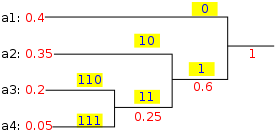
\includegraphics{Huffman.png}
\caption{Huffman tree. Source: http://en.wikipedia.org/wiki/Huffman\_coding}
\end{figure}


Notice that the symbols which occur with lower probability have longer codes and the symbols which occur with higher probability have shorter codes.

In the context of model selection, this gives you a way of picking models that regularize over some parameters. Suppose we have $m$ models $g_1(\cdot | \theta_1), ..., g_m(\cdot | \theta_m)$. The MDL for model $i$ is defined by
$$MDL = - \log g_i(X|\hat{\theta}_i) - \log f_i(\hat{\theta})$$
where $\hat{\theta}_i$ was chosen optimally to give the shortest code length and $f_i(\hat{\theta})$ is some model for $\theta$. The first term is like the MLE and provides information about the fit of the model, while the second term regularizes the complexity of the model. This corresponds tot he 2-stage MDL (see Hansen and Yu, 2001).

For the final project, we will use gMDL (where we specify a Bayesian prior on the parameters).
